\chapter{Data Processing Examples}
\label{ch:examples}

\definecolor{lgray}{gray}{0.95}

This chapter showcases a variety of results that are possible when
processing different data sets with the Stereo Pipeline. It is also a
shortened guide that shows the commands used to process specific
mission data. There is no definitive method yet for making elevation
models as each stereo pair is unique. We hope that the following
sections serve as a cookbook for strategies that will get you started
in processing your own data. We recommend that you second check your
results against another source.

\section{Guidelines for Selecting Stereo Pairs}

When choosing image pairs to process, images that are taken with
similar viewing angles, lighting conditions, and significant surface
coverage overlap are best suited for creating terrain
models. Depending on the characteristics of the mission data set and
the individual images, the degree of acceptable variation will
differ. Significant differences between image characteristics
increases the likelihood of stereo matching error and artifacts, and
these errors will propagate through to the resulting data products.

Although images do not need to be map-projected before running the
\texttt{stereo} program, we recommend that you do run {\tt cam2map}
(or \texttt{cam2map4stereo.py})
beforehand, especially for image pairs that contain large topographic
variation (and therefore large disparity differences across the
scene, e.g., Valles Marineris).  Map-projection is especially necessary
when processing \ac{HiRISE} images. This removes the large disparity
differences between \ac{HiRISE} images and leaves only the small
detail for the Stereo Pipeline to compute. Remember that \ac{ISIS}
can work backwards through a map-projection when applying the camera
model, so the geometric integrity of your images will not be sacrificed
if you map-project first.

An alternative way of map-projection, that applies to non-ISIS imagery
as well, is with the \texttt{mapproject} tool (section
\ref{mapproj-example}).

Excessively noisy images will not correlate well, so images should be
photometrically calibrated in whatever fashion suits your purposes. If
there are photometric problems with the images, those photometric
defects can be misinterpreted as topography.

Remember, in order for \texttt{stereo} to process stereo pairs in
\ac{ISIS} cube format, the images must have had SPICE data associated
by running ISIS's \texttt{spiceinit} program run on them first.

%% \subsection{Comparing Examples to your System}

%% Since our first release we re-performed some of these examples and
%% recorded their processing time so you the user can judge how long it
%% will take you. Our examples were processed on our server called
%% `Lunokhod 2'. This server is a Dell PowerEdge Rack 900 purchased in
%% late 2009. Below are its specifications:

%% \begin{center}
%% \begin{tabular}{ l | l }
%% CPU & Dual E7420 Xeon at 2.13 GHz \emph{(16 logical cores)} \\ \hline
%% FSB & 1066 MHz \\ \hline
%% L2 Cache & 8 MB \\ \hline
%% Memory & 64 GB @ 667 MHz (mis-matched?) \\ \hline
%% Storage & Local RAID5 \\ \hline
%% OS & Red Hat Enterprise Linux 5.5 \\ \hline
%% BogoMIPS & 4256 \\ \hline
%% Color & Dell Graphite \\
%% \end{tabular}
%% \end{center}

%% The times recorded are listed in wall hours and CPU hours. Wall-hours
%% are how long it took the job to complete from the user's
%% perspective. CPU-hours are how much processing time it took to
%% complete. If the job took 30 wall-minutes on a 2 core system, it spent
%% 30 minutes in CPU 1 and CPU 2. Thus, the total CPU-hours would be
%% 1. This example, though correct, is not what always happens in the
%% real world. Inefficiency with managing multiple threads or the
%% complete lack of multithreaded code will bring wall hours up to CPU
%% hours. Your required CPU hours will vary based on CPU
%% architecture. Estimating your required CPU hours for your system can
%% be done by scaling with the BogoMIPS measurements. This can be read
%% from Linux systems with the command: \texttt{cat /proc/cpuinfo}

\section{Mars Reconnaissance Orbiter HiRISE}

\ac{HiRISE} is one of the most challenging cameras to use when making 3D
models because \ac{HiRISE} exposures can be several gigabytes each. Working
with this data requires patience as it will take time.

One important fact to know about HiRISE is that it is composed of
multiple linear CCDs that are arranged side by side with some vertical
offsets. These offsets mean that the CCDs will view some of the same
terrain but at a slightly different time and a slightly different
angle. Mosaicking the CCDs together to a single image is not a simple
process and involves living with some imperfections.

One cannot simply use the \ac{HiRISE} RDR products, as they do not
have the required geometric stability.  Instead, the \ac{HiRISE}
EDR products must be assembled using \ac{ISIS} \texttt{noproj}.
The USGS distributes a script in use by the \ac{HiRISE} team that
works forward from the team-produced `balance' cubes, which provides
a de-jittered, noproj'ed mosaic of a single observation, which is
perfectly suitable for use by the Stereo Pipeline (this script was
originally engineered to provide input for SOCET SET).  However,
the `balance' cubes are not available to the general public, and
so we include a program (\texttt{hiedr2mosaic.py}, written in
\href{http://www.python.org}{Python}) that will take \ac{PDS}
available \ac{HiRISE} EDR products and walk through the processing
steps required to provide good input images for \texttt{stereo}.

The program takes all the red CCDs and projects them using the \ac{ISIS}
{\tt noproj} command into the perspective of the RED5 CCD. From there,
{\tt hijitreg} is performed to work out the relative offsets between
CCDs. Finally the CCDs are mosaicked together using the average
offset listed from {\tt hijitreg} using the {\tt handmos} command,
and the mosaic is normalized with {\tt cubenorm}.
Below is an outline of the processing.

\begin{verbatim}
    hi2isis           # Import HiRISE IMG to Isis
    hical             # Calibrate
    histitch          # Assemble whole-CCD images from the channels
    spiceinit
    spicefit          # For good measure
    noproj            # Project all images into perspective of RED5
    hijitreg          # Work out alignment between CCDs
    handmos           # Mosaic to single file
    cubenorm          # Normalize the mosaic
\end{verbatim}

To use our script, first go to the directory where you have downloaded
the HiRISE's RED EDR \texttt{IMG} files. You can run the
\texttt{hiedr2mosaic.py} program without any arguments to view a short
help statement, with the \texttt{-h} option to view a longer help statement,
or just run the program on the EDR files like so:

\begin{verbatim}
    hiedr2mosaic.py *.IMG
\end{verbatim}

If you have more than one observation's worth of EDRs in that
directory, then limit the program to just one observation's EDRs
at a time, e.g. \texttt{hiedr2mosaic.py PSP\_001513\_1655*IMG}.  If you
run into problems, try using the \texttt{-k} option to retain all of
the intermediary image files to help track down the issue.  The
\texttt{hiedr2mosaic.py} program will create a single mosaic file
with the extension \texttt{.mos\_hijitreged.norm.cub}.  Be warned that
the operations carried out by \texttt{hiedr2mosaic.py} can take many
hours to complete on the very large HiRISE images.

An example of using ASP with HiRISE data is included in the
\texttt{examples/HiRISE} directory (just type 'make' there).

\subsection{Columbia Hills}

%% \begin{tabular}{ l r c r c}
%% \textit{Prepping Files:}       & Wall Time & \texttt{+36:00:00.0} & CPU Time & \texttt{+36:00:00.0} \\
%% \textit{Processing in Stereo:} & Wall Time & \texttt{297:28:06.0} & CPU Time & \texttt{881:39:45.54} \\
%% \end{tabular}

\ac{HiRISE} observations
\href{http://hirise.lpl.arizona.edu/PSP_001513_1655}{PSP\_001513\_1655} and
\href{http://hirise.lpl.arizona.edu/PSP_001777_1650}{PSP\_001777\_1650}
are on the floor of Gusev Crater and cover the area where the \ac{MER}
Spirit landed and has roved, including the Columbia Hills.

\begin{figure}[h!]
\centering
  \subfigure[{\tt 3D Rendering}]{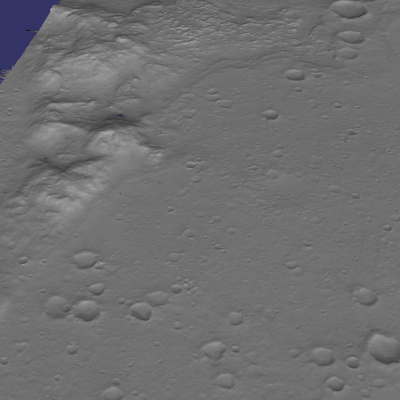
\includegraphics[width=3in]{images/examples/hirise/chills_hirise_example_400px.png}}
  \hfil
  \subfigure[{\tt KML Screenshot}]{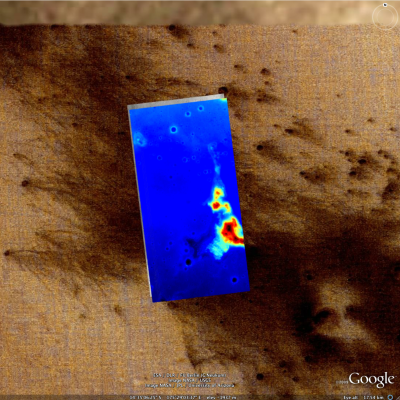
\includegraphics[width=3in]{images/examples/hirise/chills_hirise_ge_example_400px.png}}
\caption{Example output using HiRISE images PSP\_001513\_1655 and
  PSP\_001777\_1650 of the Columbia Hills.}
\label{fig:hirise_chills_example}
\end{figure}

\subsubsection*{Commands}

Download all 20 of the RED EDR \texttt{.IMG} files for each observation.
\begin{verbatim}
  ISIS 3> hiedr2mosaic.py PSP_001513_1655_RED*.IMG
  ISIS 3> hiedr2mosaic.py PSP_001777_1650_RED*.IMG
  ISIS 3> cam2map4stereo.py PSP_001777_1650_RED.mos_hijitreged.norm.cub \
                            PSP_001513_1655_RED.mos_hijitreged.norm.cub
  ISIS 3> stereo PSP_001513_1655.map.cub \
                 PSP_001777_1650.map.cub result/output
\end{verbatim}

\subsubsection*{stereo.default}

The stereo.default example file (appendix \ref{ch:stereodefault})
should apply well to HiRISE. Just set
\texttt{alignment-method} to \texttt{none} if
using map-projected imagery. If you are not using map-projected
imagery, set \texttt{alignment-method} to \texttt{homography} or
\texttt{affineepipolar}. The \texttt{corr-kernel} value can usually be
safely reduced to 21 pixels to resolve finer detail and faster
processing for images with good contrast.

\vfill

\section{Mars Reconnaissance Orbiter CTX}

\ac{CTX} is a moderate camera to work with. Processing times for
\ac{CTX} can be pretty long when using Bayes EM subpixel
refinement. Otherwise the disparity between images is relatively
small, allowing efficient computation and a reasonable processing time.

\subsection{North Terra Meridiani}

%% \begin{tabular}{l r c r c}
%% \textit{Processing in Stereo:} & Wall Time & \texttt{13:28:04.00} & CPU Time & \texttt{45:54:50.10} \\
%% \end{tabular}

In this example, we use map-projected images. Map-projecting the
images is the most reliable way to align the images for
correlation. However when possible, use non-map-projected images with
the \texttt{alignment-method affineepipolar} option. This greatly reduces
the time spent in triangulation. For all cases using linescan cameras,
triangulation of map-projected images is 10x slower than
non-map-projected images.

This example is distributed in the \texttt{examples/CTX} directory (type
'make' there to run it).

\begin{figure}[b!]
\centering
  \subfigure[{\tt 3D Rendering}]{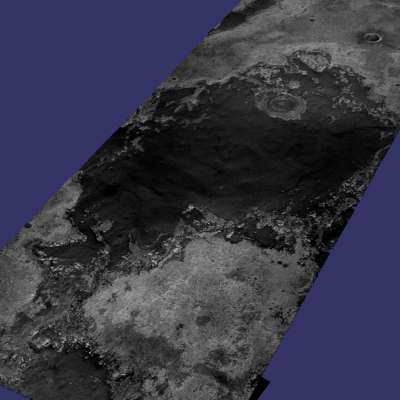
\includegraphics[width=3in]{images/examples/ctx/n_terra_meridiani_ctx_400px.png}}
  \hfil
  \subfigure[{\tt KML Screenshot}]{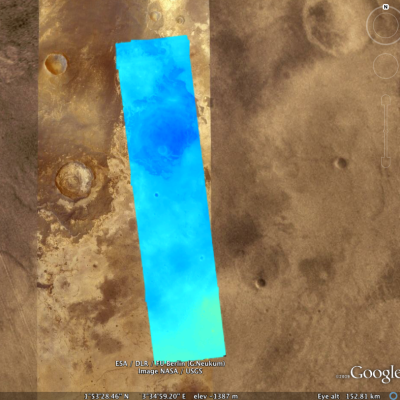
\includegraphics[width=3in]{images/examples/ctx/n_terra_meridiani_ctx_ge_400px.png}}
\caption{Example output possible with the CTX imager aboard MRO.}
\label{fig:ctx_example}
\end{figure}

\subsubsection*{Commands}

Download the \ac{CTX} images P02\_001981\_1823\_XI\_02N356W.IMG and
P03\_002258\_1817\_XI\_01N356W.IMG from the \ac{PDS}.
\begin{Verbatim}[commandchars=\\\{\}]
  ISIS 3> mroctx2isis from=P02_001981_1823_XI_02N356W.IMG to=P02_001981_1823.cub
  ISIS 3> mroctx2isis from=P03_002258_1817_XI_01N356W.IMG to=P03_002258_1817.cub
  ISIS 3> spiceinit from=P02_001981_1823.cub
  ISIS 3> spiceinit from=P03_002258_1817.cub
  ISIS 3> ctxcal from=P02_001981_1823.cub to=P02_001981_1823.cal.cub
  ISIS 3> ctxcal from=P03_002258_1817.cub to=P03_002258_1817.cal.cub
    \textnormal{you can also optionally run} ctxevenodd \textnormal{on the} cal.cub \textnormal{files, if needed}
  ISIS 3> cam2map4stereo.py P02_001981_1823.cal.cub P03_002258_1817.cal.cub
  ISIS 3> stereo P02_001981_1823.map.cub P03_002258_1817.map.cub results/out
\end{Verbatim}

\subsubsection*{stereo.default}

The stereo.default example file (appendix \ref{ch:stereodefault})
works generally well with all CTX pairs. Just set
\texttt{alignment-method} to \texttt{homography} or
\texttt{affineepipolar}.

\clearpage
\section{Mars Global Surveyor MOC-NA}

In the Stereo Pipeline Tutorial in Chapter~\ref{ch:moc_tutorial}, we
showed you how to process a narrow angle \ac{MOC} stereo pair that
covered a portion of Hrad Vallis. In this section we will show you
more examples, some of which exhibit a problem common to stereo
pairs from linescan imagers: ``spacecraft jitter'' is caused by
oscillations of the spacecraft due to the movement of other spacecraft
hardware.  All spacecraft wobble around to some degree but some are
particularly susceptible.

Jitter causes wave-like distortions along the track of the satellite
orbit in \acp{DEM} produced from linescan camera images.  This effect can
be very subtle or quite pronounced, so it is important to check your
data products carefully for any sign of this type of artifact. The
following examples will show the typical distortions created by this
problem.

Note that the science teams of \ac{HiRISE} and \ac{LROC} are actively
working on detecting and correctly modeling jitter in their respective
SPICE data. If they succeed in this, the distortions will still
be present in the raw imagery, but the jitter will no longer produce
ripple artifacts in the DEMs produced using ours or other stereo
reconstruction software.

\subsection{Ceraunius Tholus}

%% \begin{tabular}{l r c r c}
%% \textit{Prepping Files:}       & Wall Time & \texttt{00:02:42.30} & CPU Time & \texttt{00:02:42.06} \\
%% \textit{Processing in Stereo:} & Wall Time & \texttt{00:23:00.30} & CPU Time & \texttt{00:34:11.00} \\
%% \end{tabular}

Ceraunius Tholus is a volcano in northern Tharsis on Mars. It can
be found at 23.96 N and 262.60 E. This \ac{DEM} crosses the volcano's
caldera.

\begin{figure}[h]
\centering
  \subfigure[{\tt 3D Rendering}]{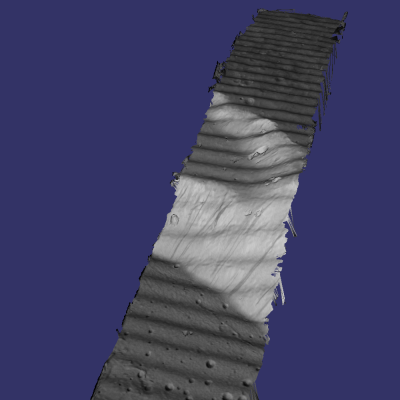
\includegraphics[width=3in]{images/examples/mocna/ceraunius_tholus_mocna_400px.png}}
  \hfil
  \subfigure[{\tt KML Screenshot}]{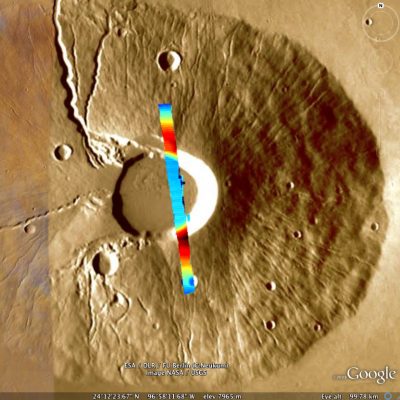
\includegraphics[width=3in]{images/examples/mocna/ceraunius_tholus_mocna_ge_400px.png}}
\caption{Example output for MOC-NA of Ceraunius Tholus. Notice the presence of severe washboarding artifacts due to spacecraft ``jitter.''}
\label{fig:mocna_ceraunius_example}
\end{figure}

\subsubsection*{Commands}

Download the M08/06047 and R07/01361 images from the \ac{PDS}.

\begin{verbatim}
  ISIS 3> moc2isis f=M0806047.img t=M0806047.cub
  ISIS 3> moc2isis f=R0701361.img t=R0701361.cub
  ISIS 3> spiceinit from=M0806047.cub
  ISIS 3> spiceinit from=R0701361.cub
  ISIS 3> cam2map4stereo.py M0806047.cub R0701361.cub
  ISIS 3> stereo M0806047.map.cub R0701361.map.cub result/output
\end{verbatim}

\subsubsection*{stereo.default}

The stereo.default example file (appendix \ref{ch:stereodefault}) works
generally well with all MOC-NA pairs. Just set \texttt{alignment-method}
to \texttt{none} when using map-projected imagery. If the images are not
map-projected, use \texttt{homography} or \texttt{affineepipolar}.

\section{Mars Exploration Rovers}\label{mer:example}

The Mars Exploration Rovers (MER) have several cameras on board
and they all seem to have a stereo pair. With ASP you are able to
process the PANCAM, NAVCAM, and HAZCAM camera imagery. ISIS has no
telemetry or camera intrinsic supports for these images. That however is
not a problem as their raw imagery contains the cameras' information in
JPL's CAHV, CAHVOR, and CHAVORE formats.

These cameras are all variations of a simple pinhole camera model so
they are processed with ASP in the \texttt{Pinhole} session instead of
the usual \texttt{ISIS}. ASP only supports creating of point
clouds. \emph{The *-PC.tif is a raw point cloud with the first 3
  channels being XYZ in the rover site's coordinate frame}. We don't
support the creation of DEMs from these images and that is left as an
exercise for the user.

An example of using ASP with MER data is included in the
\texttt{examples/MER} directory (just type 'make' there).

\subsection{PANCAM, NAVCAM, HAZCAM}

All of these cameras are processed the same way. We'll be showing 3D
processing of the front hazard cams. The only new things in the
pipeline is the new executable \texttt{mer2camera} along with the use
of \texttt{alignment-method epipolar}. This example is also provided
in the MER data example directory.

\begin{figure}[h!]
\centering
  \subfigure[{\tt Rectified Input}]{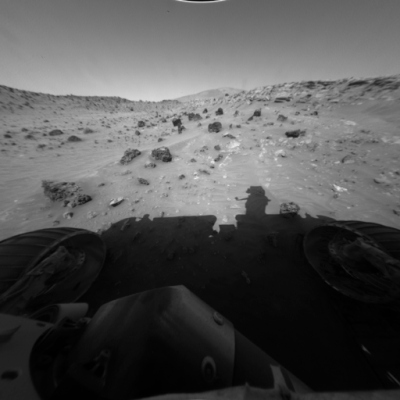
\includegraphics[width=3in]{images/examples/mer/fh01-L_sub_400px.png}}
  \hfil
  \subfigure[{\tt Output Point Cloud}]{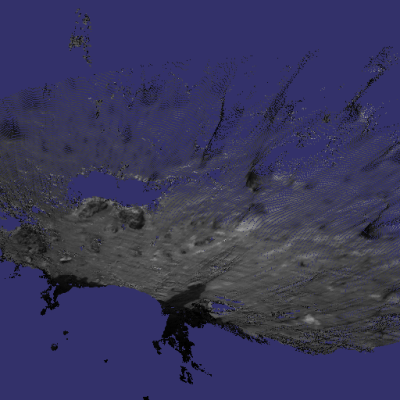
\includegraphics[width=3in]{images/examples/mer/fh01_pointcloud_400px.png}}
\caption{Example output possible with the front hazard cameras.}
\label{fig:mer_example}
\end{figure}

\pagebreak

\subsubsection*{Commands}

Download 2f194370083effap00p1214l0m1.img and
2f194370083effap00p1214r0m1.img from the \ac{PDS}.

\begin{verbatim}
  ISIS 3> mer2camera 2f194370083effap00p1214l0m1.img
  ISIS 3> mer2camera 2f194370083effap00p1214r0m1.img
  ISIS 3> stereo 2f194370083effap00p1214l0m1.img 2f194370083effap00p1214r0m1.img \
                 2f194370083effap00p1214l0m1.cahvore 2f194370083effap00p1214r0m1.cahvore \
                 fh01/fh01
\end{verbatim}

\subsection*{stereo.default}

The default stereo settings will work but change the following
options. The universe option filters out points that are not
triangulated well because they are too close \emph{robot's hardware}
or are extremely far away.

\begin{center}\begin{minipage}{5.5in}
\begin{Verbatim}[frame=single,fontsize=\small,label=additional settings for MER]
    alignment-method epipolar
    force-use-entire-range

    # This deletes points that are too far away
    # from the camera to truly triangulate.
    universe-center Camera
    near-universe-radius 0.7
    far-universe-radius 80.0
\end{Verbatim}
\end{minipage}\end{center}

\clearpage
\section{K10}\label{k10:example}

K10 is an Earth-based research rover within the Intelligent
Robotics Group at NASA Ames, the group ASP developers belong to. The
cameras on this rover use a simple Pinhole model. The use of ASP with
these cameras is illustrated in the \texttt{examples/K10} directory
(just type 'make' there).  Just as for the MER datatset (section
\ref{mer:example}), only the creation of a point cloud is supported.

\clearpage
\section{Lunar Reconnaissance Orbiter LROC NAC}
\label{lronac-example}

\subsection{Lee-Lincoln Scarp}

This stereo pair covers the Taurus-Littrow valley on the Moon where,
on December 11, 1972, the astronauts of Apollo 17 landed. However,
this stereo pair does not contain the landing site.  It is slightly
west; focusing on the Lee-Lincoln scarp that is on North Massif. The
scarp is an 80~m high feature that is the only visible sign of a deep
fault.

\begin{figure}[h!]
\centering
  \subfigure[{\tt 3D Rendering}]{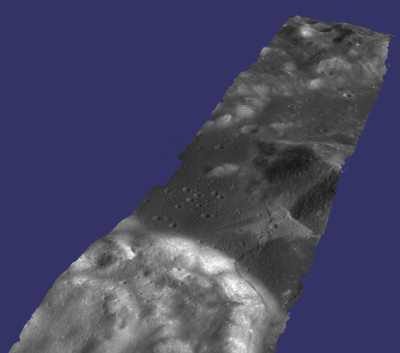
\includegraphics[width=3.8in]{images/examples/lrocna/lroc-na-example2_400px.png}}
  \hfil
  \subfigure[{\tt KML Screenshot}]{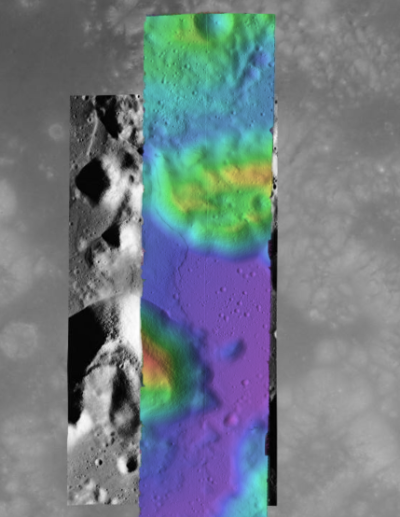
\includegraphics[width=3in]{images/examples/lrocna/lroc-na-ge_example2_400px.png}}
\caption{Example output possible with a LROC NA stereo pair, using both CCDs from each observation courtesy of the lronac2mosaic.py tool.}
\label{fig:lroc-na-example}
\end{figure}

\subsubsection*{Commands}

Download the EDRs for the left and right CCDs for observations
M104318871 and M104318871 from \url{http://wms.lroc.asu.edu/lroc/search}.
Alternatively you can search by original
IDs of 2DB8 and 4C86 in the PDS.

All ISIS preprocessing of the EDRs is performed via the
\texttt{lronac2mosaic.py} command. This runs \texttt{lronac2isis},
\texttt{lronaccal}, \texttt{lronacecho}, \texttt{spiceinit},
\texttt{noproj}, and \texttt{handmos} to create a stitched unprojected
image for a single observation. In this example we don't map-project
the images as ASP can usually get good results. More aggressive
terrain might require an additional \texttt{cam2map4stereo.py} step.

\begin{verbatim}
    ISIS 3> lronac2mosaic.py M104318871LE.img M104318871RE.img
    ISIS 3> lronac2mosaic.py M104311715LE.img M104311715RE.img
    ISIS 3> stereo M104318871LE*.mosaic.norm.cub M104311715LE*.mosaic.norm.cub \
              result/output --alignment-method affineepipolar
\end{verbatim}

\subsubsection*{stereo.default}

The defaults work generally well with LRO-NAC pairs, so you don't need
to provide a stereo.default file. Map-projecting is optional. When
map-projecting the images use \texttt{alignment-method none}, otherwise
use \texttt{alignment-method affineepipolar}. Better map-project results
can be achieved by projecting on a higher resolution elevation source
like the WAC DTM. This is achieved using the ISIS command \texttt{demprep}
and attaching to cube files via \texttt{spiceinit}'s SHAPE and MODEL
options.

\section{Apollo 15 Metric Camera Images}

\begin{tabular}{ r c r c}

\end{tabular}

Apollo Metric images were all taken at regular intervals, which means
that the same \texttt{stereo.default} can be used for all sequential
pairs of images. Apollo Metric images are ideal for stereo processing.
They produce consistent, excellent results.

The scans performed by ASU are sufficiently detailed to exhibit film
grain at the highest resolution.  The amount of noise at the full
resolution is not helpful for the correlator, so we recommend
subsampling the images by a factor of 4.

Currently the tools to ingest Apollo TIFFs into ISIS are not
available, but these images should soon be released into the PDS for
general public usage.

\subsection{Ansgarius C}

%% \begin{tabular}{ r c r c}
%% \multicolumn{3}{l}{ \emph{Prepping Files} } \\
%% Wall Time & \texttt{00:00:02.11} & CPU Time & \texttt{00:00:01.29} \\
%% \multicolumn{3}{l}{ \emph{Processing in Stereo} } \\
%% Wall Time & \texttt{01:52:23.00} & CPU Time & \texttt{21:36:07.61} \\
%% \end{tabular}

Ansgarius C is a small crater on the west edge of the far side of the
Moon near the equator. It is east of Kapteyn A and B.

\begin{figure}[h!]
\centering
  \subfigure[{\tt 3D Rendering}]{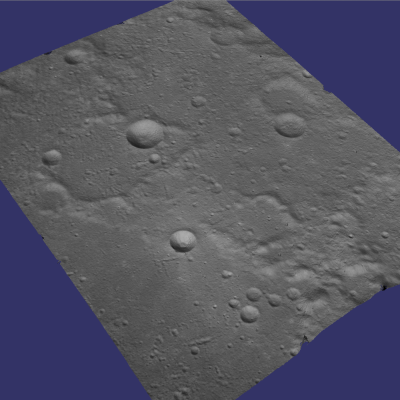
\includegraphics[width=3in]{images/examples/metric/metric_example_400px.png}}
  \hfil
  \subfigure[{\tt KML Screenshot}]{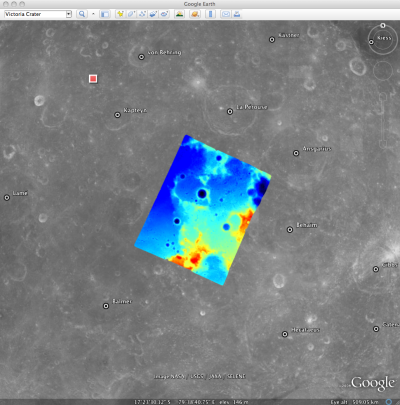
\includegraphics[width=3in]{images/examples/metric/metric_ge_example_400px.png}}
\caption{Example output possible with Apollo Metric frames AS15-M-2380 and AS15-M-2381.}
\label{fig:metric_example}
\end{figure}

\pagebreak

\subsubsection*{Commands}

Process Apollo TIFF files into \ac{ISIS}.
\begin{verbatim}
  ISIS 3> reduce from=AS15-M-2380.cub to=sub4-AS15-M-2380.cub sscale=4 lscale=4
  ISIS 3> reduce from=AS15-M-2381.cub to=sub4-AS15-M-2381.cub sscale=4 lscale=4
  ISIS 3> spiceinit from=sub4-AS15-M-2380.cub
  ISIS 3> spiceinit from=sub4-AS15-M-2381.cub
  ISIS 3> stereo sub4-AS15-M-2380.cub sub4-AS15-M-2381.cub result/output
\end{verbatim}

\subsubsection*{stereo.default}

The stereo.default example file (appendix \ref{ch:stereodefault})
works generally well with all Apollo pairs. Just set
\texttt{alignment-method} to \texttt{homography} or
\texttt{affineepipolar}.

%% \pagebreak

%% \section{MESSENGER MDIS}

%% These results are a proof of concept showing off the strength of
%% building the Stereo Pipeline on top of \ac{ISIS}. Support for processing
%% MDIS stereo pairs was not a goal during our design of the software,
%% but the fact that an MDIS camera model exists in ISIS means that
%% it too can be processed by the Stereo Pipeline.

%% For future mappers, we suggest checking out Mercury Flyby 3 data which
%% was not available at the time of this writing. Flyby 3 and Flyby 2
%% seem to have covered some of the same terrain with the narrow angle
%% camera.

%% \subsection{Wide Angle on flyby 2}

%% In most flyby imagery it is very hard to find good stereo pairs.
%% This pair was taken from a single flyby just seconds apart. Note
%% also that this pair is taken from different wavelengths (the letter
%% at the end of the filename designates the current filter being used
%% on the wide angle camera). Unfortunately there is not enough of a
%% perspective change here to make anything other than the spherical
%% surface, but that alone is still an interesting result nonetheless.

%% \begin{figure}[h!]
%% \begin{minipage}{4in}
%% 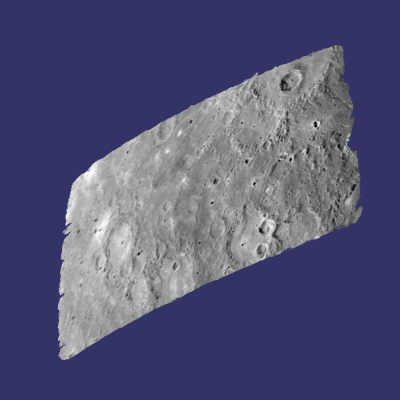
\includegraphics[width=4in]{images/examples/mdis/mdis_wide_example_400px.png}
%% \end{minipage}
%% \hfill
%% \begin{minipage}{2in}
%%   \caption{ A rough attempt at stereo reconstruction from MDIS imagery. }
%%   \label{fig:mdis_attempt}
%% \end{minipage}
%% \end{figure}

%% \subsubsection*{Commands}

%% \begin{verbatim}
%%   ISIS 3> mdis2isis from=EW0108825359A.IMG to=EW0108825359A.cub
%%   ISIS 3> mdis2isis from=EW0108825379C.IMG to=EW0108825379C.cub
%%   ISIS 3> spiceinit from=EW0108825359A.cub
%%   ISIS 3> spiceinit from=EW0108825359C.cub
%%   ISIS 3> mkdir result
%%   ISIS 3> stereo EW0108825359A.cub EW0108825379C.cub stereo/output
%% \end{verbatim}

%% \subsubsection*{stereo.default}

%% \begin{center}\begin{minipage}{5.5in}
%% \begin{Verbatim}[frame=single,fontsize=\small,label=stereo.default for MDIS]
%%     ### PREPROCESSING

%%     DO_INTERESTPOINT_ALIGNMENT 1
%%     INTERESTPOINT_ALIGNMENT_SUBSAMPLING 0
%%     DO_EPIPOLAR_ALIGNMENT 0

%%     FORCE_USE_ENTIRE_RANGE 0
%%     DO_INDIVIDUAL_NORMALIZATION 1

%%     PREPROCESSING_FILTER_MODE 2

%%     SLOG_KERNEL_WIDTH 1.5

%%     ### CORRELATION

%%     COST_BLUR 5
%%     COST_MODE 0

%%     H_KERNEL 25
%%     V_KERNEL 25

%%     H_CORR_MIN -10
%%     H_CORR_MAX 10
%%     V_CORR_MIN -2
%%     V_CORR_MAX 2

%%     SUBPIXEL_MODE 2

%%     SUBPIXEL_H_KERNEL 19
%%     SUBPIXEL_V_KERNEL 19

%%     ### FILTERING

%%     RM_H_HALF_KERN 5
%%     RM_V_HALF_KERN 5
%%     RM_MIN_MATCHES 60 # Units = percent
%%     RM_THRESHOLD 3
%%     RM_CLEANUP_PASSES 1

%%     FILL_HOLES 1

%%     ### DOTCLOUD

%%     NEAR_UNIVERSE_RADIUS 0.0
%%     FAR_UNIVERSE_RADIUS 0.0
%% \end{Verbatim}
%% \end{minipage}\end{center}

\clearpage

\section{Cassini ISS NAC}

This is a proof of concept showing the strength of building the Stereo
Pipeline on top of \ac{ISIS}.  Support for processing ISS NAC stereo pairs
was not a goal during our design of the software, but the fact that a
camera model exists in \ac{ISIS} means that it too can be processed by the
Stereo Pipeline.

Identifying stereo pairs from spacecraft that do not orbit their
target is a challenge. We have found that one usually has to settle
with images that are not ideal: different lighting, little perspective
change, and little or no stereo parallax. So far we have had little
success with Cassini's data, but nonetheless we provide this example
as a potential starting point.

\subsection{Rhea}

Rhea is the second largest moon of Saturn and is roughly a third the
size of our own Moon. This example shows, at the top right of both
images, a giant impact basin named Tirawa that is 220~miles across. The
bright white area south of Tirawa is ejecta from a new crater.  The
lack of texture in this area poses a challenge for our correlator. The
results are just barely useful: the Tirawa impact can barely be made
out in the 3D data while the new crater and ejecta become only noise.

\begin{figure}[p]
\centering
  \subfigure[{\tt Original Left Image}]{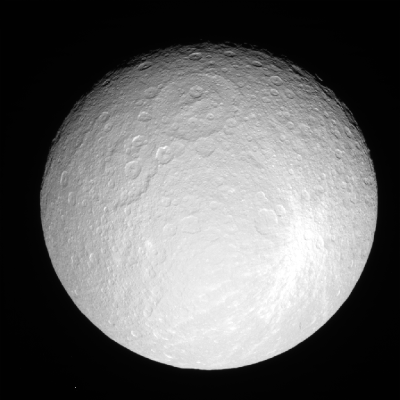
\includegraphics[width=3in]{images/examples/cassini/cassini_rhea_L_400px.png}}
  \hfil
  \subfigure[{\tt Original Right Image}]{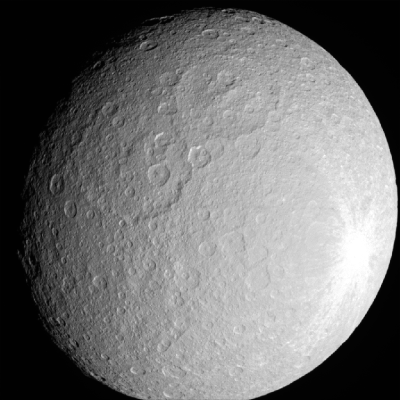
\includegraphics[width=3in]{images/examples/cassini/cassini_rhea_R_400px.png}}
  \\
  \subfigure[{\tt Map-Projected Left}]{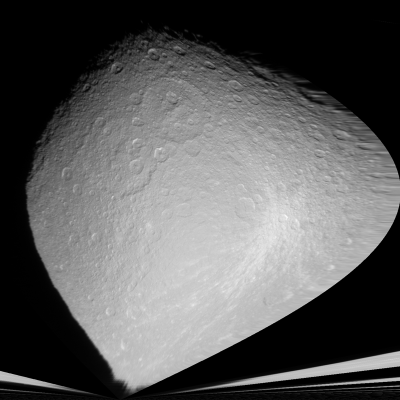
\includegraphics[width=3in]{images/examples/cassini/cassini_rhea_map_400px.png}}
  \hfil
  \subfigure[{\tt 3D Rendering}]{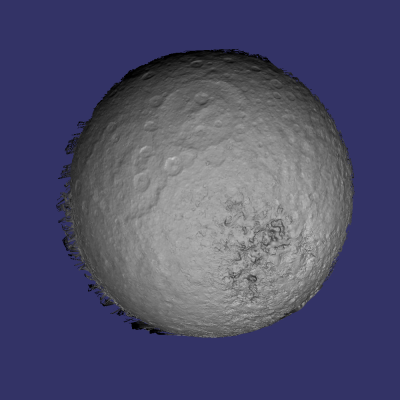
\includegraphics[width=3in]{images/examples/cassini/cassini_rhea_400px.png}}
\caption{Example output of what is possible with Cassini's ISS NAC}
\label{fig:cassini-exampe}
\end{figure}

\subsubsection*{Commands}

Download the N1511700120\_1.IMG and W1567133629\_1.IMG images and their label (.LBL) files from the \ac{PDS}.
\begin{verbatim}
  ISIS 3> ciss2isis f=N1511700120_1.LBL t=N1511700120_1.cub
  ISIS 3> ciss2isis f=W1567133629_1.LBL t=W1567133629_1.cub
  ISIS 3> cisscal from=N1511700120_1.cub to=N1511700120_1.lev1.cub
  ISIS 3> cisscal from=W1567133629_1.cub to=W1567133629_1.lev1.cub
  ISIS 3> fillgap from=W1567133629_1.lev1.cub to=W1567133629_1.fill.cub %Only one image
                                                                        %exhibits the problem
  ISIS 3> cubenorm from=N1511700120_1.lev1.cub to=N1511700120_1.norm.cub
  ISIS 3> cubenorm from=W1567133629_1.fill.cub to=W1567133629_1.norm.cub
  ISIS 3> spiceinit from=N1511700120_1.norm.cub
  ISIS 3> spiceinit from=W1567133629_1.norm.cub
  ISIS 3> cam2map from=N1511700120_1.norm.cub to=N1511700120_1.map.cub
  ISIS 3> cam2map from=W1567133629_1.norm.cub map=N1511700120_1.map.cub \
  ISIS 3>           to=W1567133629_1.map.cub matchmap=true
  ISIS 3> stereo N1511700120_1.map.equ.cub W1567133629_1.map.equ.cub result/rhea
\end{verbatim}

\subsubsection*{stereo.default}

\begin{center}\begin{minipage}{5.5in}
\begin{Verbatim}[frame=single,fontsize=\small,label=stereo.default for Cassini ISS]
    ### PREPROCESSING
    alignment-method none
    force-use-entire-range
    individually-normalize

    ### CORRELATION
    prefilter-mode 2
    prefilter-kernel-width 1.5

    cost-mode 2

    corr-kernel 25 25
    corr-search -55 -2 -5 10

    subpixel-mode 3
    subpixel-kernel 21 21

    ### FILTERING
    rm-half-kernel 5 5
    rm-min-matches 60 # Units = percent
    rm-threshold 3
    rm-cleanup-passes 1

\end{Verbatim}
\end{minipage}\end{center}

\section{Digital Globe Imagery}
\label{digital_globe_data}

Processing of Digital Globe images is described extensively in the
tutorial in chapter \ref{ch:dg_tutorial}.

\section{GeoEye and Astrium Imagery / RPC Imagery}
\label{rpc}

GeoEye provides imagery from Ikonos and the two GeoEye
satellites. Astrium provides imagery from SPOT and Pleiades
satellites. Both companies provide only Rational Polynomial Camera
(RPC) models. RPC represents four 20-element
polynomials that map geodetic coordinates to image coordinates. Since
they are easy to implement, RPC represents a universal camera model
and can be had from many imaging providers; Digital Globe also
provides them. The only downside is that it has less precision in our
opinion compared to the linear camera model provided by Digital
Globe. For GeoEye and Astrium, the only option is using RPC.

Our RPC read driver is GDAL. If the command \texttt{gdalinfo} can identify
the RPC information inside the headers of your files, ASP will likely
be able to see it as well. This means that sometimes we can get away
with only providing a left and right image, with no extra files
containing camera information. This is specifically the
case for GeoEye.

You can download an example stereo pair from GeoEye's website at
\cite{geoeye:samples}. When we accessed the site, we downloaded a
GeoEye-1 image of Hobart, Australia. As previously stated in the
Digital Globe section, these types of images are not ideal for
ASP. This is both a forest and a urban area which makes
correlation difficult. ASP was designed more for modeling bare rock
and ice. Any results we produce in other environments is a bonus but
is not our objective.

\begin{figure}[h!]
\centering
  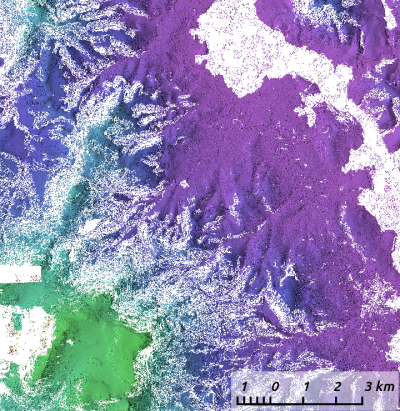
\includegraphics[width=2.0in]{images/examples/geoeye/GeoEye_ContextRender_400px.png}
  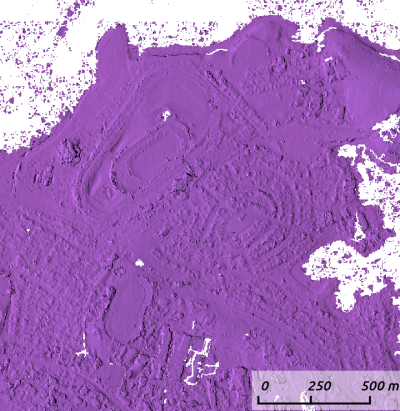
\includegraphics[width=2.0in]{images/examples/geoeye/GeoEye_CloseUp_400px.png}
  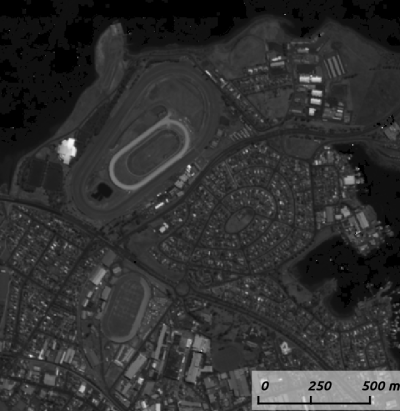
\includegraphics[width=2.0in]{images/examples/geoeye/GeoEye_CloseUpDRG_400px.png}
\caption{Example colorized height map and ortho image output.}
\label{fig:geoeye-nomap-example}
\end{figure}

\subsubsection*{Commands}

\begin{verbatim}
    > stereo -t rpc po_312012_pan_0000000.tif po_312012_pan_0010000.tif geoeye/geoeye
\end{verbatim}

In case the image files do not contain the RPC models, separate XML
files having this information need to be provided, as done for Digital
Globe images (section \ref{rawdg}).

For terrain having steep slopes, we recommend that images be map-projected
onto an existing DEM before running stereo. This is described in section
\ref{mapproj-example}.

\subsubsection*{stereo.default}

The stereo.default example file (appendix \ref{ch:stereodefault})
works generally well with all GeoEye pairs. Just set
\texttt{alignment-method} to \texttt{affineepipolar} or
\texttt{homography}.

\section{Dawn (FC) Framing Camera}

This is a NASA mission to visit two of the largest objects in the
asteroid belt, Vesta and Ceres. The framing camera on board Dawn is
quite small and packs only a resolution of 1024x1024 pixels. This means
processing time is extremely short. To its benefit, it seems that the
mission planners leave the framing camera on taking shots quite
rapidly. On a single pass, they seem to usually take a chain of FC
images that have a high overlap percentage. This opens the idea of using
ASP to process not only the sequential pairs, but also the wider
baseline shots. Then someone could potentially average all the DEMs
together to create a more robust data product.

For this example, we downloaded the images

\begin{center}
\texttt{FC21A0010191\_11286212239F1T.IMG} and
\texttt{FC21A0010192\_11286212639F1T.IMG}
\end{center}

which show the Cornelia crater. We found these images by looking at the
popular anaglyph shown on the Planetary Science Blog
\cite{planetaryblog:vesta}.

\begin{figure}[h!]
\centering
  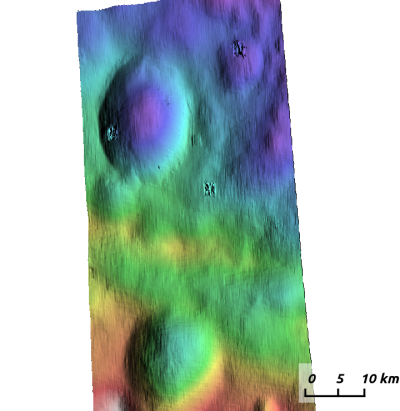
\includegraphics[width=3.0in]{images/examples/dawn/VestaDEMRender_400px.png}
  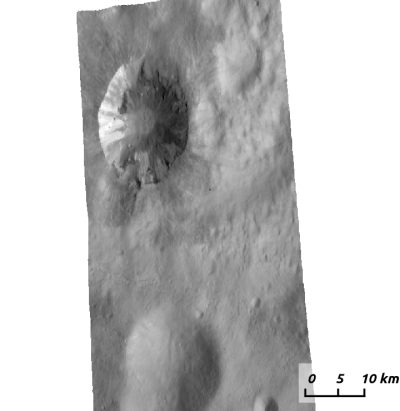
\includegraphics[width=3.0in]{images/examples/dawn/VestaDRGRender_400px.png}
\caption{Example colorized height map and ortho image output.}
\label{fig:dawn-nomap-example}
\end{figure}

\subsubsection*{Commands}

First you must download the Dawn FC images from PDS.

\begin{verbatim}
    ISIS3 > dawnfc2isis from=FC21A0010191_11286212239F1T.IMG \
                        to=FC21A0010191_11286212239F1T.cub
    ISIS3 > dawnfc2isis from=FC21A0010192_11286212639F1T.IMG \
                        to=FC21A0010192_11286212639F1T.cub
    ISIS3 > spiceinit from=FC21A0010191_11286212239F1T.cub
    ISIS3 > spiceinit from=FC21A0010192_11286212639F1T.cub
    ISIS3 > stereo FC21A0010191_11286212239F1T.cub \
                   FC21A0010192_11286212639F1T.cub stereo/stereo
    ISIS3 > point2dem stereo-PC.tif --orthoimage stereo-L.tif \
   --t_srs "+proj=eqc +lat_ts=-11.5 +a=280000 +b=229000 +units=m"
\end{verbatim}

\subsubsection*{stereo.default}

The stereo.default example file (appendix \ref{ch:stereodefault})
works well for this stereo pair. Just set
\texttt{alignment-method} to \texttt{affineepipolar} or
\texttt{homography}.


\section{ASTER Imagery}
\label{sec:aster}

In this example we will describe how to process ASTER Level 1A
VNIR imagery. We will use the dataset \texttt{030352200281191} around the
Basalt Hills quarry, near San Luis Reservoir in Northern California.

This dataset will come as a directory containing imagery and
meta-information. We use the tool \texttt{aster2asp} (section \ref{app:aster})
to parse it (also there is described the data contained in this directory):

\begin{verbatim}
  aster2asp 030352200281191 -o out
\end{verbatim}

This command will create 4 files, named \texttt{out-Band3N.tif},
\texttt{out-Band3B.tif}, \texttt{out-Band3N.xml}, and 
\texttt{out-Band3B.xml}. We refer again to the tool's documentation page
regarding details of how these files were created.

Next, we run stereo, with the RPC session, and create a DEM:
\begin{verbatim}
  stereo -t rpc --subpixel-mode 3 bout-Band3N.tif out-Band3B.tif \
     out-Band3N.xml out-Band3B.xml out_stereo/run
  point2dem -r earth --tr 0.00054 out_stereo/run-PC.tif
\end{verbatim}

The value 0.00054 is the desired output DEM resolution, specified in
degrees. It is approximately 60 meters/pixel. We chose it since the
ASTER VNIR images are about 15 meters/pixel, and running stereo is
necessarily a lossy process, so the output DEM resolution is several
times coarser than the resolution of the input imagery.

Of course, various options can be used with \texttt{stereo}, the images
can be map-projected, the cameras bundle-adjusted, etc. (see chapter
\ref{tips}).


